\subsection{Subsystem Testing}
% talks about different rigorous methods of testing the system

%\noindent FOV directivity test for range sensors, depression angle test, incoming data stream test.\\
% raise alerts if range threshold is crossed
% object detection test - range updates continuously and raises flag or interrupt if crosses below a threshold of danger
% - passing obstacle (confirm margin of safety)
% - moving obstacle
\subsubsection{Detection Threshold}
\noindent As known, there are minor dead zones in the range sensors. Therefore, to determine a safe zone range threshold, it would need to exceed the range of dead sensing. Now, there could be a way to determine that FORWARD is reading the dead zone and coordinate emergency stops based on that (although it is also important to note that an emergency stop for low range may only be necessary if S2 and S3 front-facing are dead). The detection threshold can then be hard-coded into the GNC software.\\

\noindent The first test for the obstacle detection subsystem is straightforward. It will consist of the sensor readings code uploaded to an Arduino Uno, hooked up to a laptop which rests on the seat of the rollator. The serial plotter will be open and we aim to observe changes to pitch and yaw angles as well as sensor ranges all simultaneously. This will provide a visual indication and verification that the proper decisions based on detections can be created in senior design 2. This test should work regardless of surface material and orientation of the obstacle. Therefore, it will be tested indoors in a hallway and open forum environment, outdoors in a neighborhood. The indoor test environments resemble that which FORWARD might be deployed in the medical hospital or assisted living facility, while it may also be driven around in lower calamity settings. Regardless, we will verify that ranging is independent of the environment.\\

\begin{figure}[H]
	\centering
	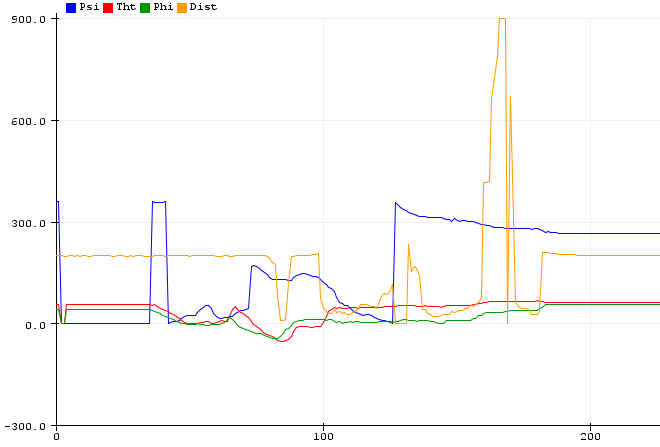
\includegraphics[width=0.7\textwidth]{./Images/serial-plotter.png}
	\caption{\label{fig:serial-plot}Euler Angles and LiDAR Distance Plot Test}
\end{figure}

% object identification test - classify obstacles and send walker into a moded resposne
% relay audio feedback to user informing them what is ahead
\subsubsection{Identification Importance}


% object avoidance test - activate feedback and update motor speeds
\subsubsection{Control Feedback}


% in SD2, will need to refine turning ratios, hazard range thresholds, and work on stretch requirements.